\documentclass[12pt,twoside]{report}
\usepackage{hyperref}
\usepackage{graphicx}
\usepackage{amsmath, amssymb}
\usepackage[table]{xcolor}
\usepackage{amssymb}
\usepackage{csquotes}
\usepackage{amsthm}
\usepackage{subdepth}
\newtheorem{theorem}{Theorem}
% Ctrl + Alt + B to compile in Atom

%%%%%%%%%%%%%%%%%%%%%%%%%%%%%%%%%%%%%%%%%%%%%%%%%%%%%%%%%%%%%%%%%%%%%%%%%%%%%

% Definitions for the title page
% Edit these to provide the correct information
% e.g. \newcommand{\reportauthor}{Timothy Kimber}
\DeclareMathOperator{\E}{\mathbb{E}}

\newcommand{\reporttitle}{Symbolic Reinforcement Learning using Inductive Logic Programming (DRAFT)}
\newcommand{\reportauthor}{Kiyohito Kunii}
\newcommand{\supervisor}{Professor Alessandra Russo}
\newcommand{\degreetype}{MSc in Computing Science}

%%%%%%%%%%%%%%%%%%%%%%%%%%%%%%%%%%%%%%%%%%%%%%%%%%%%%%%%%%%%%%%%%%%%%%%%%%%%%

% load some definitions and default packages
%%%%%%%%%%%%%%%%%%%%%%%%%%%%%%%%%%%%%%%%%
% University Assignment Title Page
% LaTeX Template
% Version 1.0 (27/12/12)
%
% This template has been downloaded from:
% http://www.LaTeXTemplates.com
%
% Original author:
% WikiBooks (http://en.wikibooks.org/wiki/LaTeX/Title_Creation)
%
% License:
% CC BY-NC-SA 3.0 (http://creativecommons.org/licenses/by-nc-sa/3.0/)
%
%
%%%%%%%%%%%%%%%%%%%%%%%%%%%%%%%%%%%%%%%%%
%----------------------------------------------------------------------------------------
%	PACKAGES AND OTHER DOCUMENT CONFIGURATIONS
%----------------------------------------------------------------------------------------
\usepackage[a4paper,hmargin=2.8cm,vmargin=2.0cm,includeheadfoot]{geometry}
\usepackage{textpos}
\usepackage[numbers]{natbib} % for bibliography
\usepackage{tabularx,longtable,multirow,subfigure,caption}%hangcaption
\usepackage{fncylab} %formatting of labels
\usepackage{fancyhdr} % page layout
\usepackage{url} % URLs
\usepackage[english]{babel}
\usepackage{amsmath}
\usepackage{graphicx}
\usepackage{dsfont}
\usepackage{epstopdf} % automatically replace .eps with .pdf in graphics
\usepackage{backref} % needed for citations
\usepackage{array}
\usepackage{latexsym}

% \usepackage[pdftex,pagebackref,hypertexnames=false,colorlinks]{hyperref} % provide links in pdf
\usepackage{hyperref}
\hypersetup{pdftitle={},
  pdfsubject={},
  pdfauthor={},
  pdfkeywords={},
  pdfstartview=FitH,
  pdfpagemode={UseOutlines},% None, FullScreen, UseOutlines
  bookmarksnumbered=true, bookmarksopen=true, colorlinks,
    citecolor=black,%
    filecolor=black,%
    linkcolor=black,%
    urlcolor=black}

\usepackage[all]{hypcap}


%\usepackage{color}
%\usepackage[tight,ugly]{units}
%\usepackage{float}
%\usepackage{tcolorbox}
%\usepackage[colorinlistoftodos]{todonotes}
% \usepackage{ntheorem}
% \theoremstyle{break}
% \newtheorem{lemma}{Lemma}
% \newtheorem{theorem}{Theorem}
% \newtheorem{remark}{Remark}
% \newtheorem{definition}{Definition}
% \newtheorem{proof}{Proof}


%%% Default fonts
\renewcommand*{\rmdefault}{bch}
\renewcommand*{\ttdefault}{cmtt}



%%% Default settings (page layout)
\setlength{\parindent}{0em}  % indentation of paragraph

\setlength{\headheight}{14.5pt}
\pagestyle{fancy}
\renewcommand{\chaptermark}[1]{\markboth{\chaptername\ \thechapter.\ #1}{}}

\fancyfoot[ER,OL]{\sffamily\textbf{\thepage}}%Page no. in the left on odd pages and on right on even pages
\fancyfoot[OC,EC]{\sffamily }
\renewcommand{\headrulewidth}{0.1pt}
\renewcommand{\footrulewidth}{0.1pt}
\captionsetup{margin=10pt,font=small,labelfont=bf}


%--- chapter heading

\def\@makechapterhead#1{%
  \vspace*{10\p@}%
  {\parindent \z@ \raggedright \sffamily
    \interlinepenalty\@M
    \Huge\bfseries \thechapter \space\space #1\par\nobreak
    \vskip 30\p@
  }}

%---chapter heading for \chapter*
\def\@makeschapterhead#1{%
  \vspace*{10\p@}%
  {\parindent \z@ \raggedright
    \sffamily
    \interlinepenalty\@M
    \Huge \bfseries  #1\par\nobreak
    \vskip 30\p@
  }}

\allowdisplaybreaks


% load some macros
% Here, you can define your own macros. Some examples are given below.

\newcommand{\R}[0]{\mathds{R}} % real numbers
\newcommand{\Z}[0]{\mathds{Z}} % integers
\newcommand{\N}[0]{\mathds{N}} % natural numbers
\newcommand{\C}[0]{\mathds{C}} % complex numbers
\renewcommand{\vec}[1]{{\boldsymbol{{#1}}}} % vector
\newcommand{\mat}[1]{{\boldsymbol{{#1}}}} % matrix


\date{June 2018}


% \newtheoremstyle{definition}[section]
\newtheorem{examp}{example}[section]


\begin{document}


% load title page
% Last modification: 2015-08-17 (Marc Deisenroth)
\begin{titlepage}

\newcommand{\HRule}{\rule{\linewidth}{0.5mm}} % Defines a new command for the horizontal lines, change thickness here


%----------------------------------------------------------------------------------------
%	LOGO SECTION
%----------------------------------------------------------------------------------------


\includegraphics[width = 4cm]{./figures/imperial}\\[0.5cm] 

\center % Center remainder of the page

%----------------------------------------------------------------------------------------
%	HEADING SECTIONS
%----------------------------------------------------------------------------------------

\textsc{\Large Imperial College London}\\[0.5cm] 
\textsc{\large Department of Computing}\\[0.5cm] 

%----------------------------------------------------------------------------------------
%	TITLE SECTION
%----------------------------------------------------------------------------------------

\HRule \\[0.4cm]
{ \huge \bfseries \reporttitle}\\ % Title of your document
\HRule \\[1.5cm]
 
%----------------------------------------------------------------------------------------
%	AUTHOR SECTION
%----------------------------------------------------------------------------------------

\begin{minipage}{0.4\textwidth}
\begin{flushleft} \large
\emph{Author:}\\
\reportauthor % Your name
\end{flushleft}
\end{minipage}
~
\begin{minipage}{0.4\textwidth}
\begin{flushright} \large
\emph{Supervisor:} \\
\supervisor % Supervisor's Name
\end{flushright}
\end{minipage}\\[4cm]


%----------------------------------------------------------------------------------------
%	FOOTER & DATE SECTION
%----------------------------------------------------------------------------------------
\vfill % Fill the rest of the page with whitespace
Submitted in partial fulfillment of the requirements for the MSc degree in
\degreetype~of Imperial College London\\[0.5cm]

\makeatletter
\@date 
\makeatother


\end{titlepage}


% page numbering etc.
\pagenumbering{roman}
\clearpage{\pagestyle{empty}\cleardoublepage}
\setcounter{page}{1}
\pagestyle{fancy}

%%%%%%%%%%%%%%%%%%%%%%%%%%%%%%%%%%%%
% \begin{abstract}
% Your abstract.
% \end{abstract}
%
% \cleardoublepage
%%%%%%%%%%%%%%%%%%%%%%%%%%%%%%%%%%%%
% \section*{Acknowledgments}
% Comment this out if not needed.
%
% \clearpage{\pagestyle{empty}\cleardoublepag e}

%%%%%%%%%%%%%%%%%%%%%%%%%%%%%%%%%%%%
%--- table of contents
\fancyhead[RE,LO]{\sffamily {Table of Contents}}
\tableofcontents

% ADD BLANK PAGE
% \clearpage{\pagestyle{empty}\cleardoublepage}
\pagenumbering{arabic}
\setcounter{page}{1}
\fancyhead[LE,RO]{\slshape \rightmark}
\fancyhead[LO,RE]{\slshape \leftmark}

%%%%%%%%%%%%%%%%%%%%%%%%%%%%%%%%%%%%
\chapter{Introduction}
\label{introduction}
% IMPERIAL LOGO
% \begin{figure}[tb]
% \centering
% 
\includegraphics[width = 0.4\hsize]{./figures/imperial}
% \caption{Imperial College Logo. It's nice blue, and the font is quite stylish. But you can choose a different one if you don't like it.}
% \label{fig:logo}
% \end{figure}
% Figure~\ref{fig:logo} is an example of a figure.

There have been successful applications of deep reinforcement learning (DRL) in a number of domains, such as video games \cite{Mnih2015}, the game of Go \cite{Silver2016} and robotics \cite{Levine2015}. However, there are still a number of issues to overcome with this method.
First, it requires a large amount of data for training the model, and the leraning process takes a long time.
Second, it is considered to be a black-box, meaning that the decision making process is unknown to the human user and therefore lacks explanation of the decision making. Third there is no thought process to the decision making, such as understanding relational representations or planning.
To tackle these problems, researchers have explored several different approaches.
One of the methods is to incorporate symbolic representations into the system to achieve more data-efficient learning \cite{Garnelo2016}. This approach is promising and shows a potential.
In this paper, we extend this approach and explore the potential of incorporating inductive logic programming into reinforcement learning to solve the above issues.
There are several advantages of symbolic reinforcement learning. First of all, the decision making mechanism is understandable by humans rather than being black-box.
Second, it resembles how humans reason. Like reinforcement learning, there are some aspects of trial-and-error in human learning, but humans exploit reasonings to efficiently learn about their surrounding or situations. They also effectively use previous experience (background knowledge) when encountering similar situations.
Finally, the recent advance of ILP research has enabled us to apply ILP in more complex situations and there are a number of new algorithms that work well in non-monotonic scenarios based on Answer Set Programmings (ASPs).

Particularly since \cite{Garnelo2016}, there have been several researches that further explored the incorporation of symbolic reasoning into DRL, but the combining of inductive logic programming and reinforcement learning has not been explored.
Because of the recent advancement of symbolic machine learning and deep reinforcement learning, a combination of both approaches would be the next fielf to explore.

In this work, our objective is to explore this new researchield and see how combination of the two different learning methods could enhance the learning capability.

In this paper, we further explore the incorporation of symbolic machine learning into reinforcement learning to achieve data-efficient learning using Inductive Learning of Answer Set Programs (ILASP), which is a state-of-art symbolic learning method that can be applied to incomplete and more complex environments.

This background report will be part of the final report and is organised as follows: In Chapter \ref{background}, the background of logic, inductive logic programming and reinforcement learning necessary for this paper are described. Chapter \ref{related_work} discusses previous research on this particular approach. Chapter \ref{project_overview} shows the tentative architecture of our new approach, using Inductive Learning of Answer Set Programs (ILASP) to generate a model of the environment. We also discuss some of the issues we currently face with the architecture and plan the implementation. Finally the ethics checklist is provided in Chapter \ref{ethics_checklist}.

\chapter{Background}
\label{background}

This chapter introduces necessary background of Inductive Logic Programming (Section \ref{ilp}) and Reinforcement Learning (Section \ref{rl}), which provide the foundations of our research.

\section{Inductive Logic Programming (ILP)}
\label{ilp}

Inductive Logic Programming (ILP) is a subfield of machine learning research area aimed at the intersection between machine learning and logic programming \cite{Muggleton1991}. The purpose of ILP is to inductively derive a hypothesis H that is a solution of a learning task, which coveres all positive examples and none of negative examples, given a hypothesis language for search space and cover relation \cite{DeRaedt1997}. ILP is based on learning from entailment, as shown in Equation \ref{ilp_equation}.

\begin{equation}
B \wedge H \models E
\end{equation}
\label{ilp_equation}

where E contains all of the positive examples (E\textsuperscript{+}) and none of the negative examples (E\textsuperscript{-}).

One of the advantage of ILP over statistical machine learning is that the hypothesis the agent learnt can be easily understood by a human, as it is expressed in first-order logic, making the learning process more transparent rather than black-box.

One of the limitations of ILP is learning efficiency. There are usually thousands or more examples in many real-world examples. Scaling ILP task to cope with large examples is a challenging task \cite{Muggleton1993}.

In this section, we briefly introduce basic logic notions, Anser set programming (ASP) and some of inductive leraning frameworks.

\subsection{Logic Basics}

%TODO Satisfiable

To compute an inference task, the syntax of the predicate logic program needs to be converted into Conjunctive Normal Form (CNF), or clausal theory, which consists of a conjunction of clauses, where a clause is disjunction of literals, and a literal can include positive literals and negative literals. A literal is either an atom \textit{p} or \textit{not p} (negation as failure).

\begin{examp} \normalfont Conjunctive Normal Form (Clausal Theory)
\begin{center}
 \textit{(~rain $\vee$ umbrella $\vee$ rain\_shoes) $\wedge$ (~sunny $\vee$ roofer)}
\end{center}
\end{examp}

A \textit{Horn clause} is a subset of CNF, which is a clause with at most one positive literal, where a \textit{definite clause} (also called a \textit{rule}) contains exactly one positive literal ($\neg$ body\textsubscript{1} $\vee$ $\neg$ body\textsubscript{2} $\vee$, ..., $\vee$ $\neg$ body\textsubscript{n} $\vee$ head), and a \textit{denial} (or a \textit{constraint}) is a clause without any positive literals ($\neg$ body\textsubscript{1} $\vee$ $\neg$ body\textsubscript{2} $\vee$, ..., $\vee$ $\neg$ body\textsubscript{n}).
A \textit{normal clause} extends Horn clause with negation as failure.

\subsection{Stable Model Semantics}

Having defined the syntax of clausal logic, we now introduce its semantics under the context of stable model. The semantics of the logic is based on the notion of interpretation, which is defined under a \textit{domain}. A domain contains all the objects that exist. It is convention to use a special interpretations called \textit{Herbrand interpretations} rather than generation interpretations.

The \textit{Herbrand domain} (a.k.a \textit{Herbrand universe}) of clause sets \textit{Th} is the set of all ground terms that are constants and function symbols appeared in \textit{Th}.

%\begin{examp} \normalfont (Herbrand Domain)
%\end{examp}
The \textit{Herbrand base} of \textit{Th} is the set of all ground predicates that are formed by predicate symbols in \textit{Th} and terms in the Herbrand domain.

%\begin{examp} \normalfont (Herbrand Base)
%\end{examp}
The \textit{Herbrand interpretation} of a set of definite clauses \textit{Th} is a subset of the Herbrand base of \textit{Th}, which is a set of ground atoms that are true in terms of interpretation.

Interpretation evaluate it to true
Interpretation evaluate it to false

A \textit{Herbrand Model} is a Herbrand interpretation if and only if a set \textit{Th} of clauses is satisfiable. In other words, a set of clauses \textit{Th} is unsatisfiable if no Herbrand model was found. The Herbrand Model is a minimum Herbrand model if and only if none of its subsets is an Herbrand model. For definite logic programs, there is a unique minimal Herbrand model (the \textit{Least Herbrand Model} \textit{M(P)} ). For normal logic programs, there may not be a least Herbrand Model.

\textit{Definite Logic Program} is a set of definite rule, and  a definite rule is of the form h $\leftarrow$ a\textsubscript{1}, ..., a\textsubscript{n}, where h , a\textsubscript{1}, ..., a\textsubscript{n} are all atoms. h is the \textit{head} of the rule and a\textsubscript{1}, ..., a\textsubscript{n} are the body of the rule.

\textit{Normal Logic Program} is a set of normal rule, and a normal rule is of the form h $\leftarrow$ a\textsubscript{1}, ..., a\textsubscript{n}, \textit{not} b\textsubscript{1}, ..., \textit{not}  b\textsubscript{n} where h is the head of the rule,
 and a\textsubscript{1}, ..., a\textsubscript{n}, b\textsubscript{1}, ..., b\textsubscript{n} are the body of the rule (both the head and body are all atoms).

To solve a normal logic program \textit{Th}, the program needs to be grounded. The \textit{grounding} of \textit{Th} is the set of all clauses that are c $\in$ \textit{Th} and variables are replaced by terms in the \textit{Herbrand Domain}.

\begin{examp} \normalfont (Grounding)

P = $\begin{cases}
	p  \leftarrow not \ q. \\
	q  \leftarrow p.
      \end{cases}$
\end{examp}
\label{grounding}

ground(P) in Example \ref{grounding} is p:- not q. and q:- p. The algorithm of grounding start with the empty program Q = \{  \} and the relevant grounding is constructed by adding to each rule R to Q given that R is a ground instance of a rule in P and their positive body literals already occurs in the in the of rules in Q. The algorithm terminates when no more rules can be added to Q.
%TODO Explain grounding in ASP context.
%The grounding of a normal logic program P can be obtained by replacing each rule in P with a ground instance of the rule, such that for each atom A in body\textsuperscript{+} (R) (TODO EXPLAIN WHAT THIS IS), already occurs in the head of another ground rule.
Not only the entire program needs to be grounded in order for ASP solver to work, and, unlike Prolog,  but also each rule must be \textit{safe}. A rule \textit{R} is safe if every variable that occurs in the head of the rule occurs at least once in body\textsuperscript{+}(R) .

Since there is no unique least Herbrand Model for a normal logic program, \cite{Gelfond1988} defined Stable Model of a normal logic program. In order to obtain the Stable model of P, P needs to be converted using \textit{Reduct} with respect to an interpretation X. First, if the body of any rule in P contains an atom which is not in X, those rules need to be removed. Second, all default negation atoms in the remaining rules in P need to be removed.

\begin{examp} \normalfont (Reduct)

X = {p}

P = $\begin{cases}
	p  \leftarrow not\ q. \\
  q  \leftarrow not\ p. \\
  r  \leftarrow p.
      \end{cases}$
\end{examp}
\label{reduct}

In the Example \ref{reduct}, P\textsuperscript{x} is {p, r $\leftarrow$ p.}.
%Any stable model is a minimal Herbrand model, and stable sets is stable models. The stable models can be found by constructing the result of the program with respect to sets of atoms X (P\textsuperscript{x} in the following 2 steps
A stable model of P is an interpretaiton X if and only if X is the unique least Herbrand Model of ground(P)\textsuperscript{x} in the logic programs.

\subsection{Anwer Set Programming (ASP) Syntax}

Answer set of normal logic program P is a stable model, and Answer Set Programming (ASP) is a normal logic program with extensions: constrains, choice rules and optimisation. ASP program consists of a set of rules, where each rule consists of an atom and literals.A literal is either an atom \textit{p} or its default negation (negation as a failure) \textit{not p} .

A Constraint of the program P is of the form $\leftarrow$ a\textsubscript{1}, ..., a\textsubscript{n}, not b\textsubscript{1}, ..., not b\textsubscript{n}, where the rule has an empty head. The constraint filters any irrelevant answer sets. When computing ground(P)\textsubscript{x}, the empty head becomes $\perp$, which cannot be in the Answer Set.
There are two types of constraints: \textit{hard constraints} and \textit{hard constraints}. Hard constraints are strictly satisfied, whereas soft constraints are must not be satisfied but the sum of the violations should be minimised when solving ASP.

Choice rule can express possible outcomes given an action choice, which is of the form
l\{h\textsubscript{1},...,h\textsubscript{m}\}u $\leftarrow$ a\textsubscript{1}, ..., a\textsubscript{n}, not b\textsubscript{1}, ..., not b\textsubscript{n} where  l and u are integers and h\textsubscript{i} for 1 $\leq$ i $\leq$ m are atoms. The head is called \textit{aggregates}.

optimisation statement is useful to order the answer sets in terms of preference, which is of the form
\#minimize[a\textsubscript{1}=w\textsubscript{1},...a\textsubscript{n}=w\textsubscript{n}] or \#maximize[a\textsubscript{1}=w\textsubscript{1},...a\textsubscript{n}=w\textsubscript{n}] where w\textsubscript{1},..., w\textsubscript{n} is an integer weight and a\textsubscript{1},...,a\textsubscript{n} is an ground atom.  ASP solvers compute the scores of the weighted sum of the sets of ground atoms based on the true answer sets, and find optimal Answer Sets which either maximise or minimise the score.

\textit{Clingo} is one of ASP modern solvers that executes the ASP program and returns answer sets of the programs (\cite{Gebser2011}), and we will use \textit{Clingo} for the implementation of this research.

%An answer set of ASP program is interpretations that make all the ruls true.
%Non-monotonicity.
TODO ASP has true, false and unknown

\subsection{ILP Under Answer Set Semantics}

There are several ILP non-monotoic learning frameworks under the Answer set semantics . We introduce two of them: \textit{Cautious Induction} and \textit{Brave Induction} (\cite{Sakama2009}), which are foundations of \textit{Learning from Answer Sets} discussed in Section \ref{section_las}.  (for other ILP frameworks, see \cite{Otero2001}, \cite{Inoue2014}, \cite{Corapi2012} and \cite{DeRaedt1997}).
\subsubsection{Cautious Induction}
% Sakama 2008 has no concept of negative examples in this paper.
Cautious Induction task is of the form $\langle$ B, E\textsuperscript{+}, E\textsuperscript{-} $\rangle$, where B is the background knowledge, E\textsuperscript{+} is a set of positive examples and E\textsuperscript{-} is a set of negative examples.

 H $\in$ ILP\textsubscript{cautious} $\langle$ B, E\textsuperscript{+}, E\textsuperscript{-} $\rangle$ if and only if  there is at least one answer set A of B $\cup$ H (B $\cup$ H is satisfiable) such that for every anser set A of B $\cup$ H: \\
$\forall$ e $\in$ E\textsuperscript{+} : e $\in$ A \\
$\forall$ e $\in$ E\textsuperscript{-} : e $\notin$ A \\

\begin{examp} \normalfont Cautious Induction (Example)

B = $\begin{cases}
	exercises  \leftarrow not \ eat\_out. \\
	eat\_out \leftarrow exercises. \\
      \end{cases}$ \\
E\textsubscript{+} = tennis \\
E\textsubscript{-} = eat\_out \\
One possible  H $\in$ ILP\textsubscript{cautious} is \{tennis$ \leftarrow$ exercises, $\leftarrow$ not tennis \}.
\end{examp}
\label{cautious_induction_example}

The limitation of Cautious Induction is that positive examples must be true for all Answer Sets and negative examples must not be included in any of the Answer Sets. These conditions may be too strict in some cases, and Cautious Induction is not able to accept the case where positive examples are true in some of the Answer Sets but not all Answer Sets of the program.

\begin{examp} \normalfont Limitation of Cautious Induction (Example)

1\{situation(P, awake), situation(P, sleep)\}1 :- person(P).

person(john).

\end{examp}
\label{limitation_cautious}

In the example \ref{limitation_cautious}, neither of situation(john, awake) or situation(john, sleep) is false in all answer sets. In this example, it only return person(john). Thus no examples could be given to learn the choice rule.

\subsubsection{Brave Induction}
Brave Induction task is of the form $\langle$ B, E\textsuperscript{+}, E\textsuperscript{-} $\rangle$ where, B is the background knowledge, E\textsuperscript{+} is a set of positive examples and E\textsuperscript{-} is a set of negative examples.
 H $\in$ ILP\textsubscript{brave} $\langle$ B, E\textsuperscript{+}, E\textsuperscript{-} $\rangle$ if and only if there is at least one answer set A of B $\cup$ H such that: \\
$\forall$ e $\in$ E\textsuperscript{+} : e $\in$ A \\
$\forall$ e $\in$ E\textsuperscript{-} : e $\notin$ A \\

\begin{examp} \normalfont Brave Induction (Example)

B = $\begin{cases}
	exercises  \leftarrow not \ eat\_out. \\
	tennis \leftarrow holiday \\
      \end{cases}$ \\
E\textsubscript{+} = tennis \\
E\textsubscript{-} = eat\_out \\
One possible  H $\in$ ILP\textsubscript{brave} is \{tennis\}, which returns \{tennis, holidy, exercises\} as Answer Sets.
\end{examp}
\label{brave_induction_example}

The limitation of Brave indction that it cannot learn constraints as shown in the example \ref{limitation_brave}.

TODO MORE EXPLANATION

\begin{examp} \normalfont Limitation of Brave Induction (Example)

B = $\begin{cases}
	1\{situation(P, awake), situation(P, sleep)\}1 \leftarrow person(P). \\
	person(C) \leftarrow super\_person(C). \\
	super\_person(john).
	\end{cases}$

In order to learn the  constraint hypothesis H = \{ $\leftarrow$ not situation(P, awake), super\_person(P)\}, it is not possible to find an optimal solution.
\end{examp}
\label{limitation_brave}

\subsection{Inductive Learning of Answer Set Programs (ILASP)}
\label{section_lasp}

\subsubsection{Learning from Answer Sets (LAS)}
\textit{Learning from Answer Sets (LAS)} was developed in \cite{Law2014} to faciliate more complex learning task that neither Cautious Induction nor Brave Induction could learn.
Examples used in LAS are \textit{Partial Interpretations}, which are of the form $\langle$ e\textsuperscript{inc}, e\textsuperscript{exc}$\rangle$. (called \textit{inclusions} and \textit{exclusions} of e respectively).  A Herbrand Interpretations extends a partial interpretation if it include all of e\textsuperscript{inc} and none of e\textsuperscript{exc}.

LAS is of the form $\langle$ B, S\textsubscript{M}, E\textsuperscript{+}, E\textsuperscript{-} $\rangle$, where B is background knowledge, S\textsubscript{M} is hypothesis space, and E\textsuperscript{+} and E\textsuperscript{-} are examples of positive and negative partial interpretations. S\textsubscript{M} consists of a set of normal rules, choice rules and constraints. S\textsubscript{M} is specified by \textit{language bias} of the learning task using \textit{mode declaration}. Mode declaration, and specifies what can occur in an hypothesis by specifying the predicate, and has two parts: \textit{modeh} and \textit{modeb}.  modeh and modeb are the predicates that can occur in the head of the rule and body of the rule respectively. Language bias is the specification of the language in the hypothesis in order to reduce search space for the hypothesis.

Given a learning task T, the set of all possible inductive solutions of T is denoted as ILP\textsubscript{LAS}(T), and a hypothesis H is an inductive solution of ILP\textsubscript{LAS}(T) $\langle$ B, S\textsubscript{M}, E\textsuperscript{+}, E\textsuperscript{-} $\rangle$ such that
\begin{enumerate}
\item H $\subseteq$ S\textsubscript{M}
\item $\forall$ e $\in$ E\textsuperscript{+} : $\exists$ A $\in$ Answer Sets(B $\cup$ H) such that A extends e
\item $\forall$ e $\in$ E\textsuperscript{-} : $\nexists$ A $\in$ Answer Sets(B $\cup$ H) such that A extends e
\end{enumerate}

%S\textsubscript{M} consists of all rules given the language bias.

\begin{examp} \normalfont LAS (Example)

TODO
%B = $\begin{cases}
%	exercises  \leftarrow not \ eat\_out. \\
%	tennis \leftarrow holiday \\
%      \end{cases}$ \\
%E\textsubscript{+} = tennis \\
%E\textsubscript{-} = eat\_out \\
%One possible  H $\in$ ILP\textsubscript{brave} is \{tennis\}, which returns \{tennis, holidy, exercises\} as Answer Sets.

\end{examp}
\label{las_example}

% Limitation of LAS??

\subsubsection{Inductive Learning of Answer Set Programs (ILASP)}

ILASP is an algorithm that is capable of solving LAS tasks, and is based on two fundamental concepts: positive solutions and violating solutions.

A hypothesis H is a positive solution if and only if
\begin{enumerate}
\item H $\subseteq$ S\textsubscript{M}
\item $\forall$ e\textsuperscript{+} $\in$ $\exists$ A $\in$ AS(B $\cup$ H) such that A extends e\textsuperscript{+}
\end{enumerate}
A hypothesis H is a violating solution if and only if
\begin{enumerate}
\item H $\subseteq$ S\textsubscript{M}
\item $\forall$ e\textsuperscript{+} $\in$ E\textsuperscript{+} $\exists$ A $\in$ Answer Sets(B $\cup$ H) such that A extends e\textsuperscript{+}
\item $\exists$ e\textsuperscript{-} $\in$ E\textsuperscript{-} $\exists$ A $\in$ Answer Sets(B $\cup$ H) such that A extends e\textsuperscript{-}\\
\end{enumerate}

Given both definitions of positive and violating solutions, ILP\textsubscript{LAS} is positive solutions that are not violating solutions.

\subsubsection{Learning from Ordered Answer Sets (LOAS)}

LOAS is an extension of ILASP by incorporating learning capability of weak constraints, is useful for modelling the agent's preferences (\cite{Law2015}).
Examples used for learning are ordered pairs of partial answer sets, which are of the form o = $\langle$ e\textsubscript{1},e\textsubscript{2} $\rangle$.  An ASP Program P \textit{bravely respects o } if and only if
\begin{enumerate}
\item $\exists$ A\textsubscript{1}, A\textsubscript{2} $\in$ Answer Sets(P) such that A\textsubscript{1} extends e\textsubscript{1}, A\textsubscript{2} extends e\textsubscript{2}, and A\textsubscript{1} $\succ$\textsubscript{P} A\textsubscript{1}
\end{enumerate}

P \textit{cautiously respects o } if and only if
\begin{enumerate}
\item $\forall$ A\textsubscript{1}, A\textsubscript{2} $\in$ Answer Sets(P) such that A\textsubscript{1} extends e\textsubscript{1}, A\textsubscript{2} extends e\textsubscript{2}, and A\textsubscript{1} $\succ$\textsubscript{P} A\textsubscript{1}
\end{enumerate}

LOAS task is of the form T = $\langle$ B, S\textsubscript{M}, E\textsubscript{+}, E\textsubscript{-}, O\textsuperscript{b},O\textsuperscript{c}$\rangle$ where O\textsuperscript{b} and O\textsuperscript{c} are brave and cautious orderings respectively, which are sets of ordering examples over set of positive partial interpretations E\textsuperscript{+}.
A hypothesis H is an inductive solution of T if and only if
\begin{enumerate}
\item H $\subseteq$ S\textsubscript{M} in ILP\textsubscript{LOAS}(T)
\item H' $\in$ ILP\textsubscript{LAS}($\langle$ B, S\textsubscript{LAS}(M\textsubscript{h}, M\textsubscript{b}), E\textsuperscript{+}, E\textsuperscript{-}$\rangle$) where H' is the subset of H without weak constraints
\item $\forall$o $\in$ O\textsuperscript{b} B $\cup$ H bravely respects o
\item $\forall$o $\in$ O\textsuperscript{c} B $\cup$ H cautiously respects o
\end{enumerate}

\subsubsection{A Context-dependent Learning from Ordered Answer Sets }
\textit{Context-dependent learning from ordered answer sets ($ILP_{LOAS}^{context}$)} is a further generalisation of ILP\textsubscript{LOAS} with \textit{context-dependent examples}.
Context-dependent examples are examples to which each unique background knowledge (context) only applies. This way the background knowledge is more structured rather than one fixed background knowledge that are applied to all examples.
Formally, partial interpretation is of the form $\langle$ e, C $\rangle$ (called \textit{context-dependent partial interpretation (CDPI)}), where \textit{e} is a partial interpretation and C is called \textit{context}, or an ASP program without weak constraints.
A \textit{context-dependent ordering example (CDOE)} is of the form $\langle$ $\langle$e\textsubscript{1}, C\textsubscript{1} $\rangle$, $\langle$ e\textsubscript{2}, C\textsubscript{2} $\rangle$$\rangle$. An APS program P \textit{bravely} respects \textit{o} if and only if
\begin{enumerate}
 \item $\exists$ $\langle$ A\textsubscript{1}, A\textsubscript{2} $\rangle$ such that A\textsubscript{1} $\in$ Answer Sets(P $\cup$ C\textsubscript{1}),  A\textsubscript{2}, $\in$ Answer Sets(P $\cup$ C\textsubscript{2}), A\textsubscript{1} extends e\textsubscript{1}, A\textsubscript{2} extends e\textsubscript{2} and A\textsubscript{1} $\prec$\textsubscript{P} A\textsubscript{2}
\end{enumerate}

 Similarly, an APS program P \textit{cautiously} respects \textit{o} if and only if
\begin{enumerate}
 \item $\forall$ $\langle$ A\textsubscript{1}, A\textsubscript{2} $\rangle$ such that A\textsubscript{1} $\in$ Answer Sets(P $\cup$ C\textsubscript{1}),  A\textsubscript{2}, $\in$ Answer Sets(P $\cup$ C\textsubscript{2}), A\textsubscript{1} extends e\textsubscript{1}, A\textsubscript{2} extends e\textsubscript{2} and A\textsubscript{1} $\prec$\textsubscript{P} A\textsubscript{2}
\end{enumerate}

$ILP_{LOAS}^{context}$ task is of the form T = $\langle$ B, S\textsubscript{M}, E\textsubscript{+}, E\textsubscript{-}, O\textsuperscript{b},O\textsuperscript{c}$\rangle$ where O\textsuperscript{b} and O\textsuperscript{c} are brave and cautious orderings respectively, which are sets of ordering examples over set of positive partial interpretations E\textsuperscript{+}.
A hypothesis H is an inductive solution of T if and only if
\begin{enumerate}
\item H $\subseteq$ S\textsubscript{M} in $ILP_{LOAS}^{context}$
\item $\forall$$\langle$ e, C$\rangle$ $\in$ E\textsuperscript{+}, $\exists$A $\exists$ A $\in$ Answer Sets (B $\cup$ C $\cup$ H) such that A extends e
\item $\forall$$\langle$ e, C$\rangle$ $\in$ E\textsuperscript{-}, $\nexists$A $\exists$ A $\in$ Answer Sets (B $\cup$ C $\cup$ H) such that A extends e
\item $\forall$o $\in$ O\textsuperscript{b} B $\cup$ H bravely respects o
\item $\forall$o $\in$ O\textsuperscript{c} B $\cup$ H cautiously respects o
\end{enumerate}

Two advantages of adding contex-dependent are it increases the efficiency of learning tasks, and more expressive structure of the background knowlege to particular examples.

\section{Reinforcement Learning (RL)}
\label{rl}
Reinforcement learning (RL) is a subfield of machine learning regarding how an agent behaves in an environment in order to maximise the total reward. As shown in Figure \ref{agent_env}, the agent interacts with an environment, and at each time step the agent takes an action and receives observation, which affects the environment state and the reward (or penalty) it receives as the action outcome. In this section, we briefly introduce the background in RL necessary for our research.

\begin{figure}[!htb]
\centering
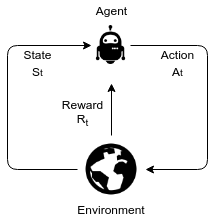
\includegraphics[width=6cm, height=6cm]{./figures/agent_env}
\caption{Agent and Environment}
\label{agent_env}
\end{figure}

\subsection{Markov Decision Process (MDP)}
An agent interacts with an environment at a sequence of discrete time step, which is a part of the sequential history of observations, actions and rewards. The sequential history is formalised as H\textsubscript{t} = O\textsubscript{1}, R\textsubscript{1}, A\textsubscript{1}, ..., A\textsubscript{t-1}, O\textsubscript{t}, R\textsubscript{t}.  A \textit{state} is a function of the history S\textsubscript{t} = f(H\textsubscript{t}), which determines the next environment.  A state S\textsubscript{t} is said to have Markov property if and only if
P[S\textsubscript{t+1} $\vert$ S\textsubscript{t}] = P[S\textsubscript{t+1} $\vert$ S\textsubscript{1}, ..., S\textsubscript{t}]. In other words, the probability of reaching S\textsubscript{t+1} depends only on S\textsubscript{t}, which captures all the relevant information from earilier history (\cite{Puterman1994}).

When an agent must make a sequence of decision, the sequential decision problem can be formalised using Markov decision process (MDP). MDPs formaly represent a fully observable environment of an agent for RL.

A MDP is of the form $\langle$ S, A, T\textsubscript{a}, R\textsubscript{a}, $\gamma$ $\rangle$ where:

\begin{itemize}
\item S is the set of finite states that is observable in the environment
\item A is the set of finite actions taken by the agent
\item T\textsubscript{a}(s, s$^\prime$) is a state transition in the form of probability matrix Pr(S\textsubscript{t+1} = s$^\prime$ $\vert$ s\textsubscript{t} = s, a\textsubscript{t} = a), which is the probablity that action a in state s at time t will result in state s$^\prime$ at time t+1.
\item R is a reward function R\textsubscript{a}(s, s$^\prime$) = $\displaystyle \E[R\textsubscript{t+1} $ $\vert$ S\textsubscript{t} = s, A\textsubscript{t} = a], the expected immediate reward that action a in state s at time t will return
\item $\gamma$ is a discount factor $\gamma$ $\in$ [0,1], which represents the preference of the agent for present rewards over future rewards
\end{itemize}

%$\displaystyle \E[R\textsubscript{t+1} \vert$ S\textsubscript{t} = s]
\subsection{Policies and Value Functions}
\textit{value functions} estimate the expected return, or expected future rewarded,  for a given action in a given state. The expected reward for an agent is dependent on the agent's action. A solution to the sequential decision problem is called a \textit{policy $\pi$}, a sequence of actions that leads to a solution.
% which is a distributin over actions given states.

The state value function v\textsubscript{$\pi$}(s) of an MDP under a policy $\pi$ is th the expected return starting from state , which is of the form:

v\textsubscript{$\pi$}(s) = $\displaystyle \E$[G\textsubscript{t} $\vert$ S\textsubscript{t} = s]

where G\textsubscript{t} = R\textsubscript{t+1} + $\gamma$R\textsubscript{t+2} + ... (the total discounted reward from t).

A policy $\pi$ is optimal if it maximises the action-value function
The transition and reward functions are not necessary to be known to compute $\pi$.

Among all possible value functions, an \textit{optimal policy $\pi^*$} is the one that maximise the total rewards in the environment.

v\textsuperscript{*}(s) = $\underset{\pi}{\max}$ v\textsubscript{$\pi$}(s)

The optimal policy $\pi$\textsuperscript{*} corresponds to v\textsuperscript{*}(s)

$\pi$\textsuperscript{*} = arg max v\textsubscript{$\pi$}(s)

%Reinforcement learning is a method to get approximated optimal solution.

TODO on-policy and off-policy learning.

A\textsubscript{t} = $\pi$(S\textsubscript{t})

One of the common possibilities is that the agent chooses an action in order to maximise the discounted sum of future rewards.

A\textsubscript{t} to maximise R\textsubscript{t+1} + $\gamma$ R\textsubscript{t+2} + $\gamma^2$ R\textsubscript{t+3} + ...

An action-value function evaluate a particular state by taking an action according the policy

q\textsubscript{$\pi$} = $\displaystyle \E[R\textsubscript{t+1} $[R\textsubscript{t+1} + $\gamma$ R\textsubscript{t+2} + $\gamma^2$ R\textsubscript{t+3} + ... $\vert$ S\textsubscript{t} = s, A\textsubscript{t} = a, A\textsubscript{t+1 } = a,]

\subsection{Model-based vs Model-free Learning}

A model M is a representation of an MDP where the state space and action space are assumed to be known. The model represents state transitions and rewards. In this case, the problem to be solved becomes a planning problem for a series of actions to achieve the agent's goal.
Most of the reinforcement learning problems are model-free learning, where M is not unknown and the agent learns to achieve the goal by solely interacting with the environment. Thus the agent knows only possible states and actions, and the transition state and reward probability functions are unknown.

The performance of model-based RL is limited to optimal policy given the model M. In other words, when the model is not a representation of the true MDP, the planning algorithms will not lead to the optimal policy, but a suboptimal policy.

One algorithm which combine both aspects of model-based and model-free learning to solve the issue of sub-optimality is called Dyna (\cite{Sutton1990}), which is shown in Figure \ref{dyna}.

\begin{figure}[!htb]
\centering
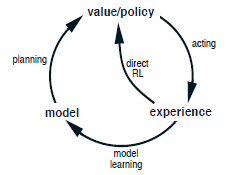
\includegraphics[width=8cm, height=6cm]{./figures/dyna}
\caption{Relationships among learning, planning and acting \ref{Montague1999}}
\label{dyna}
\end{figure}

Dyna learns a model from real experience and use the model to generate simulated experience to update the evaluation functions.

This approach is more effective because the simulated experience is relatively easy to generate compared building up real experience, thus less iterations are required.

\subsection{Temporal-Difference (TD) Learning}

To solve a MDP, one of the approaches is called Temporal-Difference (TD) Learning.
TD is an online model-free learning and learns directly from episodes of imcomplete experiences without a model of the environment.
TD updates the estimate by using the estimates of value function by bootstrap, which is formalised as

\begin{equation}
\centering
V(S\textsubscript{t}) \leftarrow V(S\textsubscript{t}) + \alpha[R\textsubscript{t+1} + \gamma V(S\textsubscript{t+1}) - V(S\textsubscript{t})]
\end{equation}

where R\textsubscript{t+1} + $\gamma$ V(S\textsubscript{t+1}) is the target for TD update, which is biased estimated of v\textsubscript{$\pi$} (S\textsubscript{t}), and $\delta$ = R\textsubscript{t+1} + $\gamma$ V(S\textsubscript{t+1}) - V(S\textsubscript{t}) is called TD error, which is the error in V(S\textsubscript{t}) available at time t+1.

Since TD methods only needs to know the estimate of one step ahead and does not need the final outcome of the episodes, it can learn online after every time step. TD also works without the terminal state, which is the goal for an agent.

TD(0) is proved to converge to v\textsubscript{$\pi$} in the table-based case (non-function approximation).
However, because bootstraping is update an estimate for an estimate, some bias is inevitable. And TD method is sensitive to initial value, (but low variance).
%\begin{equation}
%\textbf{	V(S\textsubscript{t} \leftarrow V(S\textsubscript{t} + \alpha (R\textsubscript{t+1} + \gamma V(S\textsubscript{t+1}) - V(S\textsubscript{t}))
%}\end{equation}

\subsection{Q-Learning}

Q-learning is off-policy TD learning defined in \cite{Watkins}, where the agent only knows about the possible states and actionns. The transition states and reward probability functions are unknown to the agent.
It is of the form:

\begin{equation}
Q(s\textsubscript{t},a\textsubscript{t}) \leftarrow Q(s\textsubscript{t},a\textsubscript{t}) +  \alpha(R\textsubscript{t+1} + \gamma  max (a+t) Q(s\textsubscript{t+1}, a\textsubscript{t+1}) - Q(s\textsubscript{t}, a\textsubscript{t}))
\end{equation}
%\begin{equation}

where $\alpha$ is the learning rate, $\gamma$ is a discount rate between 0 and 1. The equation is used to update the state-action value function called Q function. The function Q(S,A) predicts the best action A in state S to maximise the total cumulative rewards.
The optimal Q-function Q\textsuperscript{*}(s,a) is directly approximated by the learned action-value function Q.

% Model free can be done using Monte Carlo Policy evaluation
% One way to solve the Bellman Optimality equation is Q-leraning
% U(s) = max a Q(s,a)
% The function is estimated by Q-learning, which repeately updates Q(s,a) using the Bellman Equation.
Q-learning learns the value of its deterministic greedy policy from the experience and gradually converge to the optimal Q-function. It also explored following \textit{$\epsilon$-greedy policy}, which is a stochastic greedy policy, but with the probability of $\epsilon$, the agent chooses an action randomly instea of the greedy action.

\chapter{Related Work}
\label{related_work}
In this section, I summarise recent studies related to symbolic (deep) reinforcement learning.

 \cite{Garnelo2016} introduced Deep Symbolic Reinforcement Learning (DSRL), a proof of concept for incorporating symbolic front end as a means of converting low-dimensional symbolic representation into spatio-temporal representations, which will be the state transitions input of reinforcement learning. DSRL extracts features using convolutional neural newtworks (CNNs) \cite{LeCunL1998} and an autoencoder, which are transformed into symbolic representations for relevant object types and positions of the objects. These symbolic representations represent abstract state-space. These abstract representations are the input for the Q-learning algorithm to learn a policy on this particular state-space. DSRL was shown to outperform DRL in stochastic variant environments.
However, there are a number of drawbacks to this approach. First, the extraction of the individual objects was done by manually defined threhold of feature activation values, given that the games were geometrically simple. Thus this approach would not scale in a slightly complex game scenarios. Second, using deep neural network front-end might also cause a problem. As demonstrated in \cite{Su2017}, a single irrelevant pixel could dramatically influence the state through the change in CNNs.
While proposed method successfully used symbolic representations to achieve more data-efficient learning, there is still the potential to apply symbolic learning to those symbolic representations to further improve the learning efficiency, which is what we attemp to do in this paper.
\cite{Garcez2018} further explored this symbolic abstraction approach by incorporating the relative position of each object with respect to every other object rather than absolute object position. They also assign priority to each Q-value function based on the relative distance of objects from an agent.

\cite{Zambaldi2018} added relational reinforcement learning, a classical subfield of research aiming to combining reinforcement learning with relational learning or Inductive Logic Programming,  which added more abstract planning on top of DSRL approach. The new mode was then applied to much more complicate game environment than that used by \cite{Garnelo2016}.

%They incorporated a deep RL with architectural inductive biases
%structured representations of the game, and relatioal reasoning.

%The use of symbolic representations to achieve data-efficient learning was traditionally discussed in relational reinforcement learnign (RLL).

This idea of adding planning capability align with our approach of using ILP to improve a RL agent. In this paper, we explore how to effectively learn the model of the environment and effectively use it to facilitate data-efficient learning and transfer learning capability.

%Transparency and interpretable capability of the model is another important aspect for machine learning applications.

%XXX[Programmati...] developed a programmatically interpretable reinforcement learning which finds a policy that can be represented in a human-readable programming language.

%The history of data-efficient learning

Another approach for using symbolic reinforcement learning is storing heuristics expressed by konwledge bases [\cite{Apeldoorn2017}].  An agent lerans the concept of \textit{Hierarchical Knowledge Bases (HKBs)} [which is defined in more details in \cite{Apeldoorn2016} and \cite{Apeldoorn}] at every iteration of training, which contains multiple rules (state-action pairs).  The agent then is able to decide itself when it should exploit the heuristic rather than the state-action pairs of the RL using  \textit{Strategic Depth}. This approach effectively uses the heuristic knowledge bases, which acts as a sym-symbolic model of the game.

Another field related to our research is the combining of ASP and RL. The original concept of combining ASP and RL was in \cite{Ferreira2017}, where they developed an algorithm that efficiently finds the optimal solution of an MDP of non-stationary domains by using ASP to find the possible trajectories of an MDP. This approach focused more on efficient update of the Q function rather than inductive learning. In order to find stationary sets, an extension of ASP called BC\textsuperscript{+}, an action language,  was used. BC\textsuperscript{+} can directly translate the agent's actions into ASP form, and provide sequences of actions in Answer Sets.

ASP BC\textsuperscript{+} translation was done manually.

%Incorporation of logic into reinforcement learning dates back to the study of relational reinforcement learning,

%There are a number of research conducted in applying DNN to symbolic reasoning.
%[From GamePlay to Symbolic Reasoning]

\chapter{Project Overview}
\label{project_overview}

\section{Proposed Architecture}
\label{proposed_architecture_section}

The proposed tentative architecture is shown in Figure \ref{proposed_architecture}. The overall architecture is based on Sutton's Dyna architecture (\cite{Sutton1990}), which combined both model-free learning and model-based learning. What is different from Dyna is the way we generate the model of the environment, which is explained in the following subsections.

\begin{figure}[!htb]
\centering
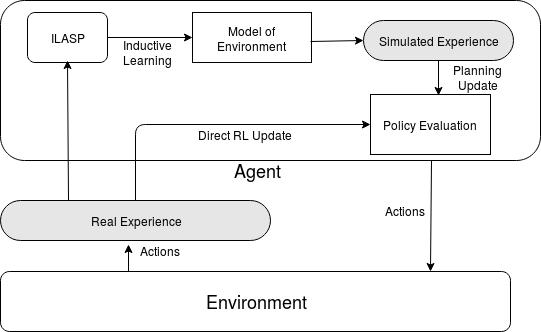
\includegraphics[width=15cm, height=9cm]{./figures/ILASRL}
\caption{Proposed reinforcement learning architecture. ILASP learns to generate a model and updates based on the interaction with the environment, which is used to facilite the policy evaluation. }
\label{proposed_architecture}
\end{figure}

\subsection{ASP Representation Generation}

At the first stage,  the input of real experience needs to be converted in ASP form, which can be used to execute the inductive learning in ILASP. The input used in ILASP is state transition, reward and action of the agent, which can be directly converted using a simple mapping table or an action language (such as BC\textsuperscript{+} as used in \cite{Ferreira2017}). The following ASP input is what is sent to ILASP. \\


agent\_at\_before(cell(X,Y), T).

agent\_at\_after(cell(X,Y), T).

reward(R, T).

action(A, T).

\subsection{Model Generation and Update using ILASP}

Once the input of the real experience is converted into ASP syntax, the agent should learn the following definition of the model of the environment using ILASP. \\

valid\_move(C, T):- link(C, T).
\\
link(C2, T):- agent\_at(C1, T), adjacent(C0, C2), not obstacle(C0, C2).\\
%state\_transition(C1, C2, T2):-
%  agent\_at\_before(C1, T1),
%  agent\_at\_after(C2, T2).\\
agent\_at(C, T):- agent\_at\_after(C, T) \\

The background knowledge is empty, and there are only positive examples in learning this task. Each example contains a different transition history of the agent. Inclusions are valid moves and exclusions are invalid moves. Learning valid\_move is the same as learning the rule of the games (the model of the environment), and it is updated as the agent explores in the environment.

In addition to the rules of the game, learning the following concepts will be crucial for transfer learning, as these concepts will be applicable to any types of game environment.  \\

adjacent(C1, C2):- cell(C1), cell(C2). \\
%obstacle(C1, C2):- enemy(C1, C2). \\
obstacle(C1, C2):- wall(C1, C2). \\
wall(C1, C2):- agent\_at\_before(C1, T1), agent\_at\_after(C1, T2) \\
enemy(C1, C2):- agent\_at\_before(C1, T1), agent\_at\_after(C2, T2), reward(R), R $<$ -100 \\

where it is assumed that the reward of -100 means losing the game or losing the agent's life. Once the agent has learned the concept of the game, it knows how to avoid an obstacle in an adjacent cell in a new environment. Figure \ref{grid_world} illustrates this transfer capability.

\begin{figure}[!htb]
\centering
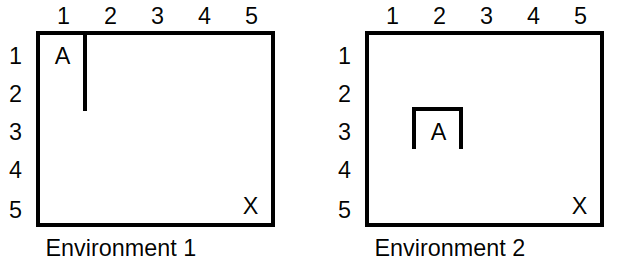
\includegraphics[width=10cm, height=5cm]{./figures/grid_world}
\caption{Simple Grid World to highlight transfer capability }
\label{grid_world}
\end{figure}

If the agent A learnt the concept \textit{adjacent} in Environment 1, the agent could reason (have a policy), for example, "if the adjacent cell is a wall, moving into that cell is an invalid move", "if the adjacent cell is an enemy, moving into that cell will incur a negative reward". These learnt policies could immediately be used in a new environment (e.g Environment 2), even though the agent's coordinates position is different from that in previous environment (e.g Environment 1).
\subsection{Generation of Simulated Experience}
Assuming the model is  a true representation of the partial environment, we can generate simulated experience to update the Q function. The simulated experience is cheaper than real experience, which should contribute to efficient learning. However Dyna architecture is known to lead to sub-optimal policy when the model is not accurate, and the solution to this problem needs to be considered further.

An alternative to using simulated experience is to directly update state representations. Once the concept "adjacent"  was learnt from a real experience, it could be incorporated in a state.

In addition, when the environment changes during the exploration, the agent should generalise its internal model to cope with the new environment in two different but similar environments.  As a result the agent's model becomes more general which covers both games. Thus in theory, the agent should still be able to achieve more efficient learning from the model-based learning, facilitating the transfer learning.
Implementation of exactly how the model is generalised will be further investigated.

\section{Further Research and Plan}
\label{research_plan}
The next phase of the research is further research on the proposed architecture, implementation and experiments.

\subsection{Further Research}
The proposed architecture is not finalised and will be reviewed regularly as we do more research.
More research needs to be devoted to finalising the overall architecture, and the following issues in particular need to be considered.
\begin{itemize}

\item Further investigation of whether ILASP can learn the concept of adjacent, which is crucial concept to know in any environment.
\item How to generalise the agent's model when the environment changes. The new environment could be very similar to the previous one, or could be a completely different environment thus the agent should create a new internal model rather than generalising the existing model.
\item The current proposed architecture is based on Dyna with simulated experiences. However, this might not be the best overall architecture, and the feasibility of using simulated experience with the learnt model with ILASP needs to be further investigated.

\item Possibility of using other representational concepts such as \textit{Predictive Representations of State} or \textit{Affordance} \cite{Sridharan2017} for the agent's learning task. These concept have not been considered at the moment, but could help better transfer learning.

\item Preparation for a backup plan in case ILASP approach does not work, so that the researchs feasible within 3 months of the researcheriod.

\end{itemize}

\subsection{Experiment Implementation}

Once the architecture is decided, we will implement it using Python and ILASPv3.1.0 (Clingo) \cite{Law2017}, and compare the performance with other learning methods using a game platform called GVG-AI Framework.

Other learning methods to be compared as benchmarks will be Q-Learning and Deep Q-Learning since these methods are widely used in other related works. Other symbolic-based approaches could also be compared as an extension. The two main measurements for the performance of our new architecture are learning efficiency and transfer learning capability as stated in the Introduction.

GVG-AI Framework was created for the General Video Gamea AI Competition \footnote{http://www.gvgai.net/}, a game environment for an agent that should be able to play a wide variety of games without knowing which games are to be played.
The underlying language is the Video Game Definition Language (VGDL), which is a high-level description language for 2D video games providing a platform for computational intelligence research (\cite{Schaul2013}).

% \section{Contribution}
%
% To my knowledge, this is the first time that both symbolic learning method is incorporated into a reinforcement learning to facilitate learning process
%
% \section{Methods}


\chapter{Ethics Checklist}
\label{ethics_checklist}

{
\renewcommand*{\arraystretch}{1.3}
\begin{longtable}{ |p{13.2cm}|p{0.6cm}|p{0.6cm}| }
\hline
 & \bf Yes & \bf No \\
\hline

\multicolumn{3}{|l|}{\cellcolor{green!25}\bf Section 1: HUMAN EMBRYOS/FOETUSES} \\
\hline

Does your project involve Human Embryonic Stem Cells? & & \checkmark\\
\hline

Does your project involve the use of human embryos? & & \checkmark\\
\hline

Does your project involve the use of human foetal tissues / cells? & & \checkmark\\
\hline

\multicolumn{3}{|l|}{\cellcolor{green!25}\bf Section 2: HUMANS} \\
\hline

Does your project involve human participants? & & \checkmark\\
\hline

\multicolumn{3}{|l|}{\cellcolor{green!25}\bf Section 3: HUMAN CELLS / TISSUES} \\
\hline

Does your project involve human cells or tissues? (Other than from “Human Embryos/Foetuses” i.e. Section 1)? & & \checkmark\\
\hline

\multicolumn{3}{|l|}{\cellcolor{green!25}\bf Section 4: PROTECTION OF PERSONAL DATA} \\
\hline

Does your project involve personal data collection and/or processing? & & \checkmark\\
\hline

Does it involve the collection and/or processing of sensitive personal data (e.g. health, sexual lifestyle, ethnicity, political opinion, religious or philosophical conviction)? & & \checkmark\\
\hline

Does it involve processing of genetic information? & & \checkmark\\
\hline

Does it involve tracking or observation of participants? It should be noted that this issue is not limited to surveillance or localization data. It also applies to Wan data such as IP address, MACs, cookies etc. & & \checkmark\\
\hline

Does your project involve further processing of previously collected personal data (secondary use)? For example Does your project involve merging existing data sets? & & \checkmark\\
\hline

\multicolumn{3}{|l|}{\cellcolor{green!25}\bf Section 5: ANIMALS} \\
\hline

Does your project involve animals? & & \checkmark\\
\hline


\multicolumn{3}{|l|}{\cellcolor{green!25}\bf Section 6: DEVELOPING COUNTRIES} \\
\hline

Does your project involve developing countries? & & \checkmark\\
\hline

If your project involves low and/or lower-middle income countries, are any benefit-sharing actions planned? & & \checkmark\\
\hline

Could the situation in the country put the individuals taking part in the project at risk? & & \checkmark\\
\hline

\multicolumn{3}{|l|}{\cellcolor{green!25}\bf Section 7: ENVIRONMENTAL PROTECTION AND SAFETY} \\
\hline

Does your project involve the use of elements that may cause harm to the environment, animals or plants? & & \checkmark\\
\hline

Does your project deal with endangered fauna and/or flora /protected areas? & & \checkmark \\
\hline

Does your project involve the use of elements that may cause harm to humans, including project staff? & & \checkmark\\
\hline

Does your project involve other harmful materials or equipment, e.g. high-powered laser systems? & & \checkmark\\
\hline


\multicolumn{3}{|l|}{\cellcolor{green!25}\bf Section 8: DUAL USE} \\
\hline

Does your project have the potential for military applications? & & \checkmark\\
\hline

Does your project have an exclusive civilian application focus? & & \checkmark\\
\hline

Will your project use or produce goods or information that will require export licenses in accordance with legislation on dual use items? & & \checkmark\\
\hline

Does your project affect current standards in military ethics – e.g., global ban on weapons of mass destruction, issues of proportionality, discrimination of combatants and accountability in drone and autonomous robotics developments, incendiary or laser weapons? & & \checkmark\\
\hline

\multicolumn{3}{|l|}{\cellcolor{green!25}\bf Section 9: MISUSE} \\
\hline

Does your project have the potential for malevolent/criminal/terrorist abuse? & & \checkmark\\
\hline

Does your project involve information on/or the use of biological-, chemical-, nuclear/radiological-security sensitive materials and explosives, and means of their delivery? & & \checkmark\\
\hline

Does your project involve the development of technologies or the creation of information that could have severe negative impacts on human rights standards (e.g. privacy, stigmatization, discrimination), if misapplied? & \checkmark& \\
\hline

Does your project have the potential for terrorist or criminal abuse e.g. infrastructural vulnerability studies, cybersecurity related project? & & \checkmark\\
\hline

\multicolumn{3}{|l|}{\cellcolor{green!25}\bf Section 10: LEGAL ISSUES} \\
\hline

Will your project use or produce software for which there are copyright licensing implications? & \checkmark& \\
\hline

Will your project use or produce goods or information for which there are data protection, or other legal implications? & & \checkmark\\
\hline

\multicolumn{3}{|l|}{\cellcolor{green!25}\bf Section 11: OTHER ETHICS ISSUES} \\
\hline

Are there any other ethics issues that should be taken into consideration? & & \checkmark \\
\hline

\end{longtable}
}

%%%%%%%%%%%%%%%%%%%%%%%%%%%%%%%%%%%%
% \chapter{Contribution}


% %%%%%%%%%%%%%%%%%%%%%%%%%%%%%%%%%%%%
% \chapter{Experimental Results}
%
%
% %%%%%%%%%%%%%%%%%%%%%%%%%%%%%%%%%%%%
% \chapter{Conclusion}

% Further research
% probabilistic inductive logic programming instead of ASP.

%% bibliography
\bibliography{references}
\bibliographystyle{ieeetr}

\end{document}
